\section{\scAssesmentHeader{Канады}}


% \subsection{\scAssesmentBuildingClass}
% % 
% \subsection{\scAssesmentBuildingMetrics}

% ##########-----Регулирование


\subsection{\scAssesmentBuildingLaw}
% 
Нормативная документация для Арктических зон Канады:
\begin{enumerate}[1.]
    \item National Building Code of Canada 2020 --- Национальный строительный кодекс Канады 2020.
    \item Canada building Code in the Context of Climate Change, Adaptation, and Sustainability --- Строительный кодекс Канады в контексте изменения климата, адаптации и устойчивого развития.
\end{enumerate}

% ##########-----Опыт


\subsection{\scAssesmentExp}

В канадской Арктике жильё представлено каркасными домами усадебного типа в стационарных постройках. Кочевники используют палатки и традиционные способы организации быта.
В проектировании и строительстве прослеживаются тенденции на включение бытовых процессов в алгоритм принятия решений при формировании функционально-планировочной организации жилья
и интеграцию опыта коренного населения в технологии строительства в Арктике.
Так, в проекте ARCTIC FOOD NETWORK\footnote{рус. Арктическая продовольственная сеть} \cite{2012_nomads_Canada_AFN}, в программу эксплуатации территории включаются сезонность добычи продовольственных ресурсов, на основе которой выстраивается градостроительное решение на уровне субъекта (уровень схем территориального планирования в терминологии актуального на период исследования российского законодательства \cite{law_RU_GradoCodex}).
Решение направлено на объединение молодого населения на основе традиционного образа жизни с современным переосмыслением, отраженного в рационе коренных жителей Северной Америки инуитов\footnote{отечественному читателю также известных, как <<эскимосы>>}, связанным с промыслом (Рисунок \ref{fig:ch01_s10_sci_AFN01_calendar}).

% \clearpage
\begin{figure}
    \centering
    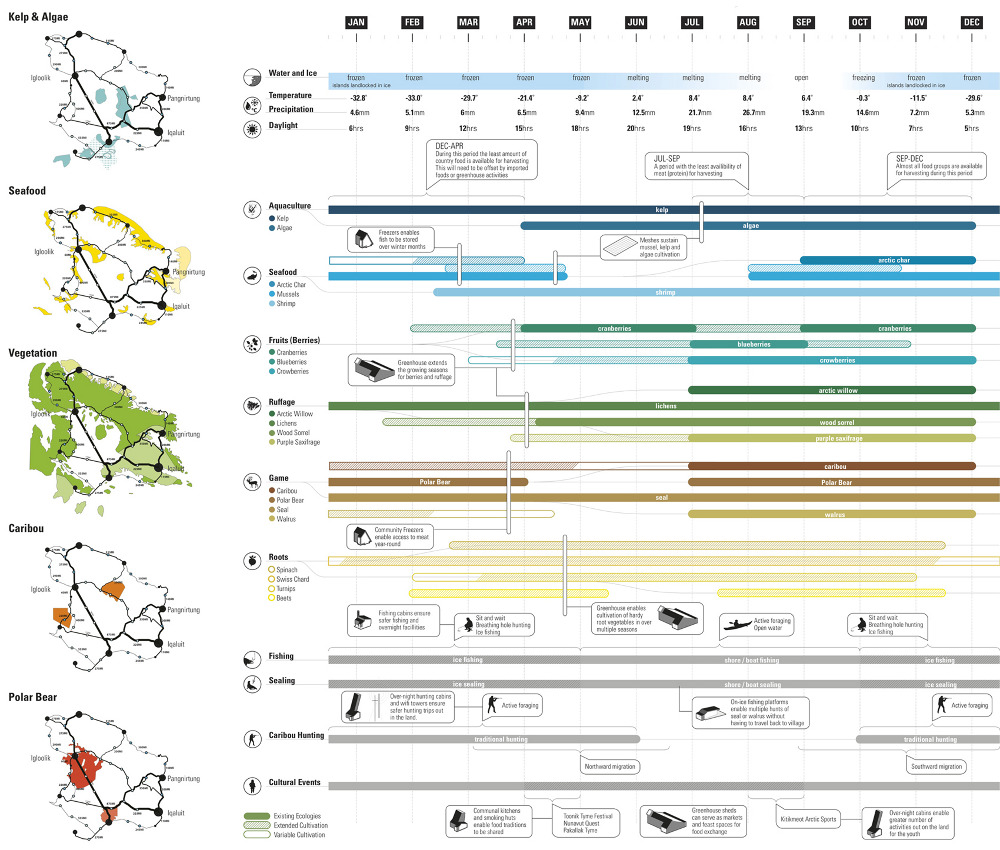
\includegraphics[width=\textwidth]{assets/figures/ch01_s10_sci_AFN01_calendar.png}
    \caption{Календарь проекта, показывающий существующую и проектную сезонность традиционных продуктов питания (графика разработана Lateral Office)}
    \label{fig:ch01_s10_sci_AFN01_calendar}
  \end{figure}

Традиционный рацион инуитов, который сосредоточен на охоте и рыболовстве, постепенно подвергается риску из-за притока пищевых продуктов, произведенных с Юга,
что приводит к увеличению уровня ожирения и диабета. Воздействие такого рациона на здоровье усиливается на Севере из-за высокой стоимости доставки свежих продуктов и более здоровой пищи.
Типичная продовольственная корзина в Нунавуте вдвое дороже аналогичной на Юге Канады, а уровень жизни и зарплаты часто ниже.
Арктическая продовольственная сеть удовлетворяет острую потребность в региональной сети арктических ферм, морозильных камер, и узлах-стоянках.
Сеть окружает большую часть бассейна Фокс в Нунавуте, Канада, ареал разнообразной дикой природы, вдоль побережья Баффиновой Земли и около 30 000 Нунавуммиут.

% \clearpage
\begin{figure}
    \centering
    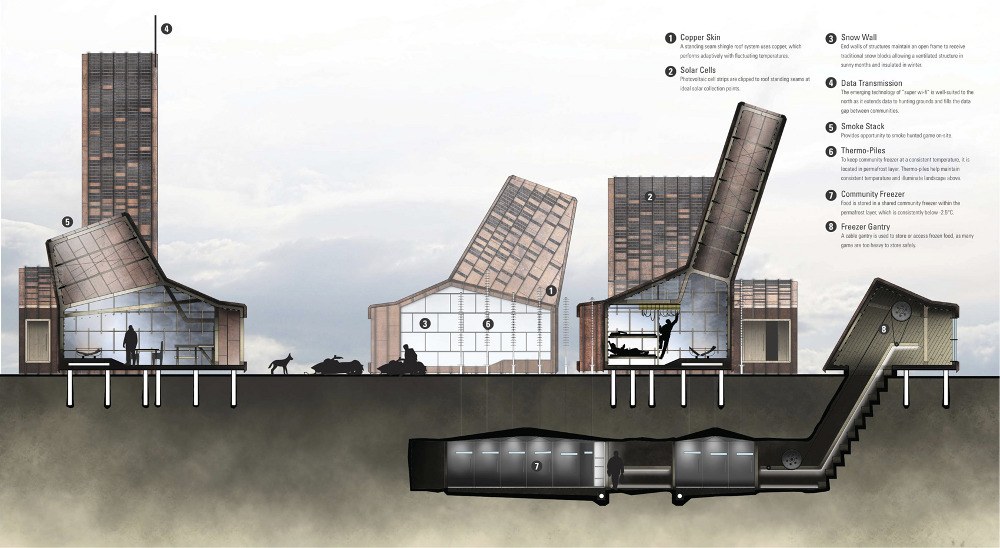
\includegraphics[width=\textwidth]{assets/figures/ch01_s10_sci_AFN01_nodeSection.png}
    \caption{Узел модулей  с кабинами, кухнями и подземными морозильными камерами (графика разработана Lateral Office)}
    \label{fig:ch01_s10_sci_AFN01_nodeSection}
  \end{figure}

Сеть состоит из того, что разработчики из Lateral Office называют навесами, сетками и полюсами, которые относятся к набору уникально интегрированных элементов,
объединяющих архитектуру, ландшафт и технологии. Проект сети - это распределённые узлы регионального сельского хозяйства,
сезонных мест стоянки, центров передачи данных и станций экологического управления. В дополнение к обеспечению безопасной продовольственной и туристической сети,
AFN стремится объединить новые технологии с традиционными практиками для поддержки развивающейся экономики 21-го века.


Таким образом, этот проект наиболее комплексно воплощает все традиционные подходы и адаптации к условиям Арктики,
рассмотренные в предшествующем разделе и реализует эти подходы как на градостроительном уровне, так и в архитектурном проектировании и инженерных решениях.
В этом проекте применяются также узлы примыкания, основанные на традиционных примыканиях в конструктивной схеме инуитского каноэ для промысла,
что является примером тенденции адаптивности инженерных решений к пользователям, создание привычных, дружественных местному коренному населению, методов возведения и обслуживания.

